\section{PSPACE}
\label{3DPSPACE}
In this section we show the PSPACE-completeness of 3D push-pull puzzles with equal push and pull strength. We will prove hardness by a reduction from TQBF. The TQBF problem asks whether, given a set of variables $\{x_1, x_2, \ldots x_n, y_1, y_2, \ldots y_n\}$ and a boolean forumla $\theta(x_1, \ldots x_n, y_1 \ldots y_n)$ in conjuctive normal form with exactly three variables per clause, the quantified boolean formula $\forall y_1 \exists x_1 \forall y_2 \exists x_2 \ldots \theta(x_1, \ldots x_n, y_1, \ldots y_n)$ is true.

We introduce a gadget called the 4-toggle and use it to simulate Quantified Boolean Formulas\cite{NPBook}. We construct the 4-toggle gadget in 3D push-pull block puzzles, completing the reduction. In particular we prove 3D Push1-Pull1 with thin walls is PSPACE-complete and 3D Push$i$-Pull$j$, for all positive $i=j$, is PSPACE-complete. A gap between NP and PSPACE still remains for 3D puzzles with different pull and push values, as well as 2D puzzles. 

We will refuce from TQBF by using the 4-toggle to construct a 2-toggle with many locks, which will be used to construct an alternating quantifier chain, as well as a clause gadget.
%\xxx{we can actually get something like all values where pull < 2push using the hypercube construction, but it's hard to describe and doesn't cover everything.}

\subsection{Toggles}
We define an $n$-toggle to be a gadget which has $n$ internal pathways and can be in one of two internal states, $A$ or $B$. Each pathway has a side labeled $A$ and another labeled $B$. When the toggle is in the $A$ state, the pathways can only be traversed from $A$ to $B$ and similarly in the $B$ state they can only be traversed from $B$ to $A$. Whenever a pathway is traversed, the state of the toggle flips.

\begin{figure}[!ht]
\centering
\begin{subfigure}[t]{0.45\textwidth}
  \centering
    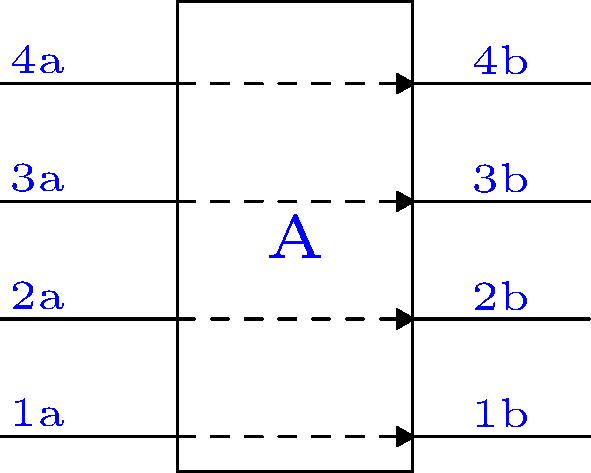
\includegraphics[width=0.8\textwidth]{Abstract4ToggleA}
    \caption{4-Toggle in state $A$. Here we can only follow the paths from left to right.}
    \label{fig:Abstract4ToggleA}
\end{subfigure}
\begin{subfigure}[t]{0.45\textwidth}
  \centering
    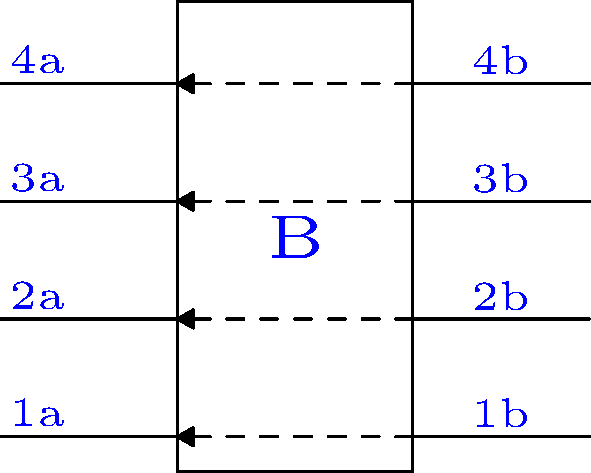
\includegraphics[width=0.8\textwidth]{Abstract4ToggleB}
    \caption{4-Toggle in state $B$. The direction of the paths through the toggle are flipped.}
    \label{fig:Abstract4ToggleB}
\end{subfigure}
\caption{Diagrams of the two possible states of a 4-Toggle.}
\end{figure}

\begin{figure}[!ht]
\centering
\begin{subfigure}[t]{0.45\textwidth}
  \centering
    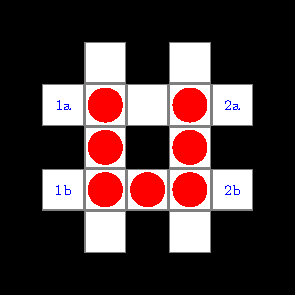
\includegraphics[width=0.8\textwidth]{2Toggle}
    \caption{2-Toggle in state $A$. The arrows indicate the transition to state $B$.}
    \label{fig:2toggleA}
\end{subfigure}
\begin{subfigure}[t]{0.45\textwidth}
  \centering
    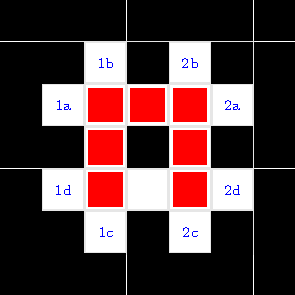
\includegraphics[width=0.8\textwidth]{2ToggleB}
    \caption{2-Toggle in state $B$.}
    \label{fig:2toggleB}
\end{subfigure}
    \begin{subfigure}[t]{0.45\textwidth}
  \centering
    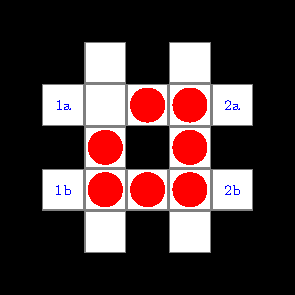
\includegraphics[width=0.8\textwidth]{broken2Toggle}
    \caption{2-Toggle in one of four broken states.}
    \label{fig:broken2toggle}
    \end{subfigure}
  \begin{subfigure}[t]{.45\textwidth}
  \centering
    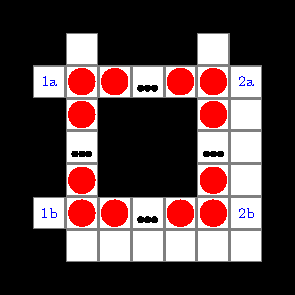
\includegraphics[width=.8\textwidth]{2ToggleK}
    \caption{Construction of a 2-toggle when the robot can push or pull multiple blocks.}
    \label{fig:2ToggleK}
    \end{subfigure}
    \caption{2-Toggles constructed in a push-pull block puzzle.}
\end{figure}

Figure~\ref{fig:2toggleA} acts as a 2-toggle. The locations $1a$, $1d$, $2a$, and $2d$, are all entrances and exits to the 2-toggle, while $1b$ connects directly to $1c$, and $2b$ connects directly to $2c$. Notice that there is a single block missing from the ring of eight blocks. When the missing block is on top, as diagrammed, it will represent state $A$, and when it is on the opposite side, we call it state $B$. Notice that in state $A$, it is impossible to enter through entries $1d$ or $2d$. When we enter in the $1a$ or $2a$ sides, we can follow the moves in the series of diagrams to exit the corresponding $1d$ or $2d$ side, leaving the gadget in the $B$ state. One can easily check that the gadget can only be left in either state $A$, $B$, or a broken state as seen in Figure~\ref{fig:broken2toggle}. Notice that in the broken state, every pathway except the one just exited is blocked. If we enter through that path, it is in exactly the same state as if it had been in an allowed state and entered through the corresponding pathway normally. For example, in the diagram one can only enter through $1d$ and after doing so it is the same as entering in path $1d$ on a 2-toggle in state $B$. Thus the broken state is never more useful for solving the puzzle and can be safely ignored.

\begin{figure}[!ht]
  \centering
  \begin{subfigure}[t]{.45\textwidth}
    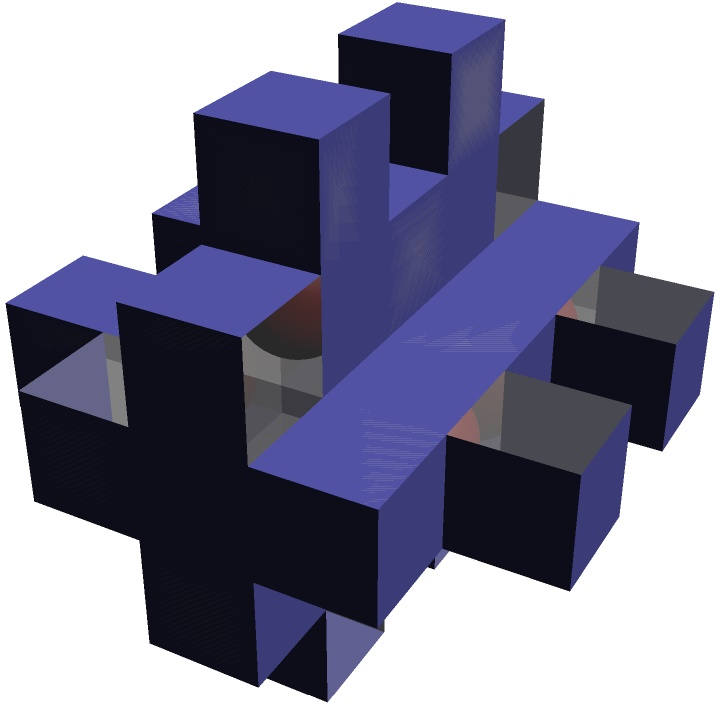
\includegraphics[width=\linewidth]{4ToggleNoConnections.jpg}
    \caption{Diagram of a 4-toggle showing impassible surfaces.}
    \label{fig:4Toggle3D}
%    \includemedia[width=0.3\linewidth,]{}{4Toggle.pdf}
  \end{subfigure}
  \hfill
  \begin{subfigure}[t]{.45\textwidth}
    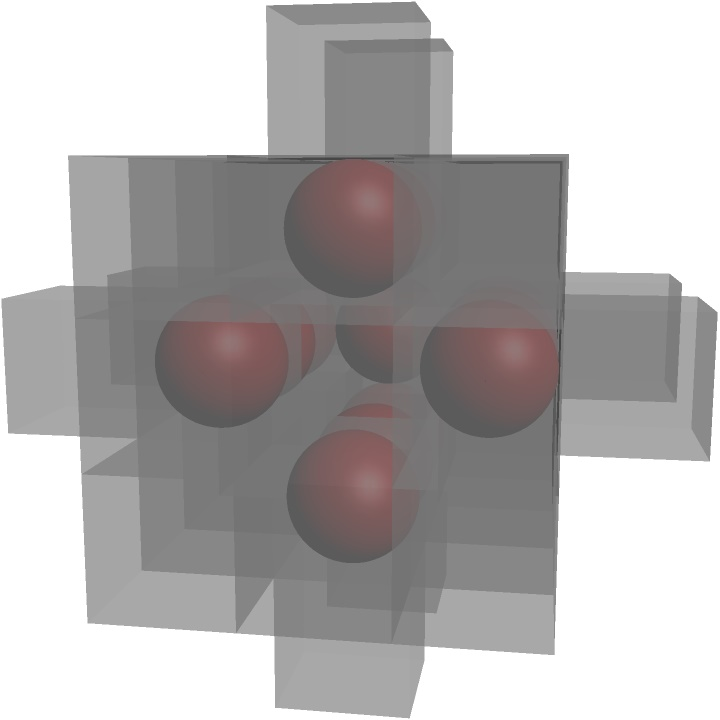
\includegraphics[width=\linewidth]{4ToggleBasic.jpg}
    \caption{Diagram of the internals of a 4-toggle.}
    \label{fig:4Toggle3DBasic}
  \end{subfigure}
  \caption{3D diagrams of 4-toggles. Red spheres are blocks and blue surfaces are impassable.}
\end{figure}

To construct a 4-toggle we essentially take two copies of the 2-toggle, rotate them perpendicular to each other in 3D, and let them overlap on the central axis. See Figure~\ref{fig:4Toggle3D}. We still interpret the lack of blocks in the same positions as in the 2-toggle as states $A$ or $B$. Now we have four different paths which function the same as the ones described above. Similar arguments show the broken states of the 4-toggle also don't matter.

For Push1-Pull1, this construction requires thin walls, as shown in Figure~\ref{fig:4Toggle3D}, since the exit pathways from $1b$, $2b$, $3b$ and $4b$ must pass immediately next to each other. For Push$k$-Pull$k$, with $k > 1$, thin walls are not necessary, since the exit pathways are separated from each other.
\subsection{Locks}


A 2-toggle and lock is a gadget consisting of a 2-toggle and a separate pathway. Traversing the separate pathway is only possible if the 2-toggle is in a specific state, and the traversal does not change the internal state of the 2-toggle. The 2-toggle functions exactly
as described above.

This gadget can be implemented using a 4-toggle by
connecting the $3B$ and $4B$ entrances of the 4-toggle with an additional corridor, as shown in Figure~\ref{fig:LockA}.
Traversing the resultant full pathway, from $3A$ to $3B$ to $4B$ to $4A$, is possible only if the initial
state of the 4-toggle is $A$, and will leave the 4-toggle in state $A$. In addition, a partial traversal,
such as from $3A$ to $3B$ and back to $3A$, does not change the internal state. The two unaffected
pathways of the toggle, $1$ and $2$, continue to function as a 2-toggle.

\begin{wrapfigure}{r}{0.45\textwidth}
  \centering
%  \begin{subfigure}[t]{0.45\textwidth}
%    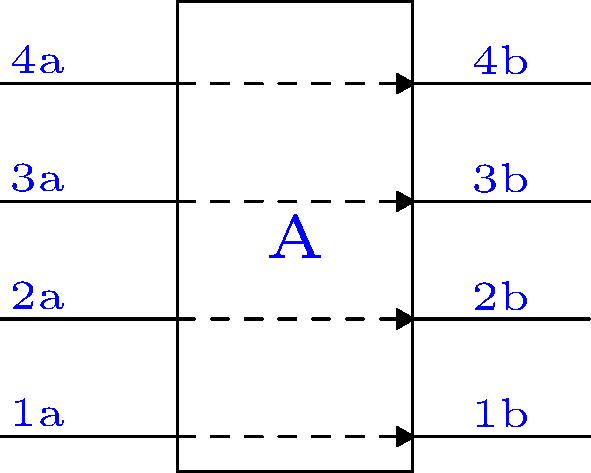
\includegraphics[width=\textwidth]{Abstract4ToggleA}
%    \caption{Representation of a 4-toggle in state $A$. }
%    \label{fig:4Toggle3D}
%  \end{subfigure}
%  \hfill
%  \begin{subfigure}[t]{0.45\textwidth}
    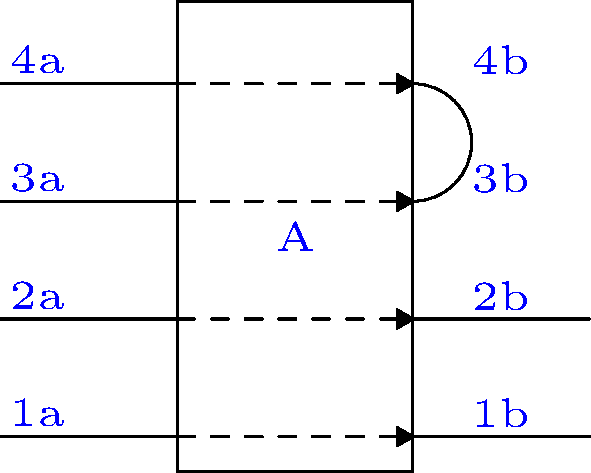
\includegraphics[width=.4\textwidth]{LockB}
    \caption{Diagram of a lock. The $3a$ to $4a$ traversal is only possible in state $A$ and returns the toggle to state $A$.}
    \label{fig:LockA}
%  \end{subfigure}
%  \caption{}
\end{wrapfigure}

A 2-toggle and lock can be extended to a 2-toggle with many locks. The 2-toggle with many locks is a gadget consisting of a 2-toggle
and any number of separate pathways. The 2-toggle still functions as described above.
Each pathway may be set up to be passable if and only if the toggle is in state $A$, or passable if and only if the toggle is in state $B$. 

This is
implemented using one 2-toggle and lock per separate pathway needed. As shown in Figure~\ref{fig:LockBlock}, there are 2
pathways which run through the entire 2-toggle and many locks gadget: the 1 pathway, and the 2 pathway. 
By choosing 2-toggles and lock gadgets that are initially passable or initially unpassable, and orienting them all so that 
their 2-toggles are all passable at once, we can create a 2-toggle and many locks with an arbitrary arrangement of locks with 
either corespondence to the state of the 2-toggle.
\begin{figure}[hb]
\centering
    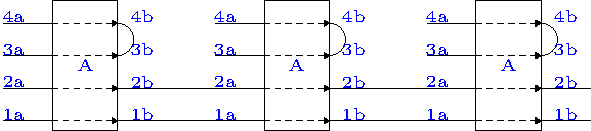
\includegraphics[width=0.9\textwidth]{LockBlock}
    \caption{A 2-toggle and many locks.}
    \label{fig:LockBlock}
\end{figure}

When the 2-toggle and many locks is traversed, all of the internal locks' states flip, rendering the gadget passable in the opposite direction, and switching the passibility and impassibility of all of the external pathways.

\subsection{Quantifiers}

We will construct a series of gadgets that will allow us to simulate quantintifiers in a boolean formula.

\subsubsection{Binary Counter}

Universal quantifiers must iterate through all possible combinations of values that they can take. In this section we construct a gadget that runs though all the states of its subcomponents as the robot progresses through the gadget. This construction will serve as the base for our universal quantifiers.

\begin{figure}[h!]
\centering
    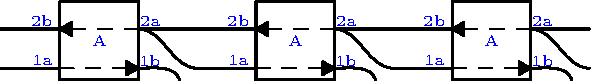
\includegraphics[width=.9\textwidth]{BinaryCounter}
    \caption{The central portion of a three bit binary counter made from 2-toggles.}
    \label{fig:BinaryCounter}
\end{figure}
  
We now define a binary counter. The binary counter has a fixed number of internal bits.
Whenever the binary counter is traversed in the forwards direction, the binary number
formed by the internal bits increases by one and the robot leaves via one of the exits.
If the binary counter is traversed in the reverse direction, the internal value is reduced by
one. If the binary counter is partially traversed, but then the robot leaves via its initial entrance,
the internal value does not change.

The binary counter is implemented as a series of 2-toggles, as shown in Figure~\ref{fig:BinaryCounter}.
The entrance pathway is connected to the 2-toggle's $1A$ and $2B$ entrances. The $1B$ exit from the 2-toggle
will exit from the entire binary counter. The $2A$ exit will continue on to the next 2-toggle,
attaching to that toggle's $1A$ and $2B$ entrances. This will continue for every toggle down the line, except
that the last toggle's $2A$ exit signals an overflow and exits from the counter.

To see that this produces the desired effect, identify a toggle in state $A$ as a $0$ bit, and a toggle in state
$B$ as a $1$ bit. Let the entrance toggle's bit be the least significant bit, and the final toggle be the
most significant. When the robot enters the binary counter in the forwards direction, it will flip
the state of every toggle it passes through. When it enters a toggle that is initially in state $B$, and thus whose
bit is $1$, it will flip the state/bit and proceed to the next toggle, via the $2B - 2A$ pathway. When it
encounters a toggle that is initially in state $A$ / bit $0$, it will flip the state/bit and exit via the $1A - 1B$
pathway. Thus, the overall effect on the bits of the binary counter is to change a sequence of bits ending at the
least significant bit from $01..11$ to $10..00$, where the entrance is at the left.
This has the effect of increasing the value of the binary counter by one.

We will not examine the reverse transitions or rigorously complete the binary counter here, 
as we do not use it directly in the final construction. 

\subsubsection{Existential Quantifier}
We now define an existential gadget. An existential gadget is like a 2-toggle and many locks, except that instead of a
2-toggle, it has a single pathway which is always passable in both directions, and upon traversing the pathway
the robot may or may not change the internal state of the 2-toggle and many locks, as it chooses. The variable is 
considered true if the 4-toggles in the lock block are in state $A$ and false if they are in state $B$. This gadget
is shown in Figure~\ref{fig:Existential}.

\begin{figure}[h!]
\centering
    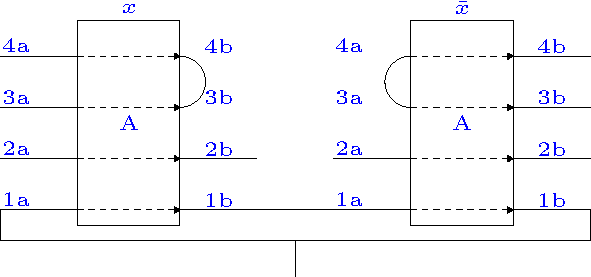
\includegraphics[width=0.9\textwidth]{existentialGadget}
    \caption{An existential gadget is simply a lock block with a number of copies equal to the number of times the corresponding variable occurs in the formula.}
    \label{fig:Existential}
\end{figure}


\subsubsection{Alternating Quantifier Chain}
\begin{figure}[h!]
\centering
    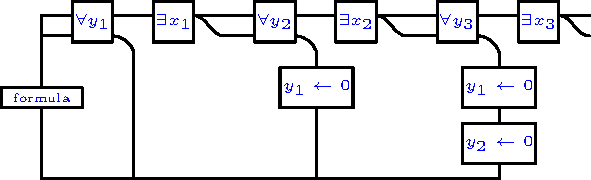
\includegraphics[width=0.9\textwidth]{QuantifierChain}
    \caption{A segment of the alternating quantifier chain. Each square represents the 2-toggle part of a 2-toggle and many locks.}
    \label{fig:QuantifierChain}
\end{figure}

We now define an alternating quantifier chain, as shown in Figure~\ref{fig:QuantifierChain}. An alternating quantifier chain implements a series of
alternating existential and universal variables, as well as external literal pathways, which may be traversed
if and only if their corresponding variables are set to a prespecified value.

Traversing the quantifier chain
repeatedly in the primary direction will cycle the universal variables through all $2^n$ possible settings.
Upon each traversal, an initial sequence of the universal variables will have their values flipped.
During the traversal, the robot will have the option to set a series of corresponding existential variables to whatever value they wish. These comprise the existentials nested within the universal variables whose values were flipped.

Traversing  the quantifier chain in the reverse direction is only possible if the robot enters
via the lowest order universal toggle whose setting is $1$. The traversal will go back one setting in the
sequence of possible settings of the universal variables, and allow the robot to set all existential variables
corresponding to altered universal variables arbitrarily. No other existential variables can be changed.

There is also a special exit, the overflow exit, which can only be
reached after all of the universal variable settings have been traversed. This is the target location for the robot.

A quantifier chain is implemented much like a binary counter, with some additions. Every universal variable will be represented by a 2-toggle and many locks, where individual locks will serve as a literal. The 2-toggles are hooked up in the same manner as the 2-toggles in a binary counter gadget. This forces the 2-toggle and many locks gadgets to be set to the corresponding values in the simulated binary counter.

The next addition is the existential variables, which consist of existential gadgets placed just after the $2A$
exits of each universal variable,
and just before the $1A$ and $2B$ entrances of the the next universal variable, as shown
in Figure~\ref{fig:QuantifierChain}.

One portion of the apparatus which has not been analyzed thus far is the potential for the robot to re-enter the chain of existentials
via a different exit pathway than the one just exited. This would be problematic if the robot re-entered via a universal gadget it had not just exited,
both because the robot should not be able to take any action other than reversing its prior progress, 
decrementing the binary counter/universal quantifiers. Problems would also arrise if the robot got access to any existential quantifiers 
it did not just traverse.

After a traversal, the universal quantifiers have the settings $\ldots??10\ldots00$, where the lowest significance $1$ is 
on the pathway just exited.
To prevent the robot from re-entering via any pathway other than the one just exited, we add a series of locks to each exit that are only passable
if all lower-significance universal toggles are in state $0$, as shown in Figure~\ref{fig:QuantifierChain}.
This does not impede the exit that the robot uses initially, since all
lower-significance universal toggles are indeed $0$. These locks do prevent re-entry into any higher-significance universal toggles, since the
lock corresponding to the lowest-significance $1$ will be closed. The robot cannot re-enter via any toggle that is in state $0$,
due to the arrangement of the toggle pathways. Thus, the unique re-enterable pathway is the lowest-significance toggle in state $1$, as desired.

\subsection{Clause Gadget}
We construct a clause gadget by putting lock pathways of three 2-toggle with many locks in parallel, as we did with Set-Verify gadgets in Figure~\ref{fig:NPClauseGadget}. Each of these paths can be traversed only if the corresponding variable has been seti to true, or to false, depending on the orientation of that particular lock. Since they are in parallel, only one needs to be passable for the robot to be able to continue on to the next clause.

\subsection{Beginning and End Conditions}
The overall progression of the robot through the puzzle starts with the quantifier chain.
The robot increments the universal variables and sets the appropriate existential variables arbitrarily, 
then traverses a series of claise gadgets to verify that the TQBF formula represented by those clauses 
is true under that setting of the variables. Then, the robot cycles around to the quantifier chain, and repeats.

At the beginning of this procedure, the robot must be allowed to set all of the existential variables arbitrarily.
To ensure this, we will set up the quantifier gadget in the state $01 .. 11$, with all variables set to $1$
except the highest order one.  The highest order variable will be special, and will not be used in the $3CNF$
formula. The initial position of the robot will be at the entrance to the quantifier gadget. This will allow
the robot to flip every universal in the quantifier gadget, from $01 .. 11$ to $10 .. 00$, and accordingly
set every existential variable arbitrarily. To force the robot to go forward through the quantifier gadget
instead of going backwards through the clause chain, we will add a literal onto the end of the formula gadget
which is passable if and only if the highest order variable is set to $1$.

After this set up, the robot will progress through the loop consisting of the quantifier gadget and the
formula gadget, demonstrating the appropriate existential settings for each assignment of the universal
quantifiers.

At each point in this process, the robot has the option to proceed through this cycle backwards, as is
guaranteed by the reversibility of the game. However, at no point does proceeding in the reverse direction
give the robot the ability to access locations or set toggles to states that it could not have performed
when it initially encountered the toggles or locations. Thus, any progression through the states of the
alternating quantifier chain must demonstrate a TQBF solution to the formula given.

After progressing through every possible state of the universal quantifiers, the universals will be in the
state $11 .. 11$. At this point, the robot may progress through the quantifier gadget and exit via its special
pathway,
the carry pathway of the highest order bit. This special pathway will lead to the goal location of the puzzle.
Thus, only by traversing the quantifier - formula loop repeatedly, and demonstrating the solution to the TQBF
problem,
will the robot be able to reach the goal. The robot may reach the goal if and only if the corresponding quantified
boolean formula is true.

Thus, TQBF can be reduced to the problem of solving a Push$k$-Pull$k$ game in three dimensions. This implies that Push$k$-Pull$k$ is PSPACE-hard.
Since Push$k$-Pull$k$ has a polynomial-size state, the problem is in NPSPACE, and therefore in PSPACE. So it is PSPACE-complete.
